\documentclass{beamer}
\usepackage[utf8]{inputenc}
\usepackage[T1]{fontenc}
\usepackage[swedish,english]{babel}
\usepackage{color}
\usepackage{xcolor}
\usepackage{amssymb}
\usepackage{amsmath}
\usepackage{ae}
\usepackage{units}
\usepackage{caption}
\usepackage{subcaption}
\definecolor{olive}{RGB}{0,139,69}
\usetheme{Pittsburgh}
\usecolortheme[RGB={0,139,69}]{structure}
\setbeamertemplate{navigation symbols}{}
\setbeamersize{text margin left=2mm, text margin right=2mm}

%% Skriv \frametitle{foo} för rubrik på en slide
%% \color{olive}{} för text i den gröna färgen
%% Figurer behöver ej vara floats, dvs \begin{figure} ej nödvändigt
%%
%%
%%

\begin{document}

\section{Presentation}

\frame{
  \begin{center}

    \textcolor{olive}{{
        \Large Väderparametrars inverkan på \\ energiförluster i en fastighet
      } \\
      - en studie av värmeflöden
    }

    \vskip10pt

    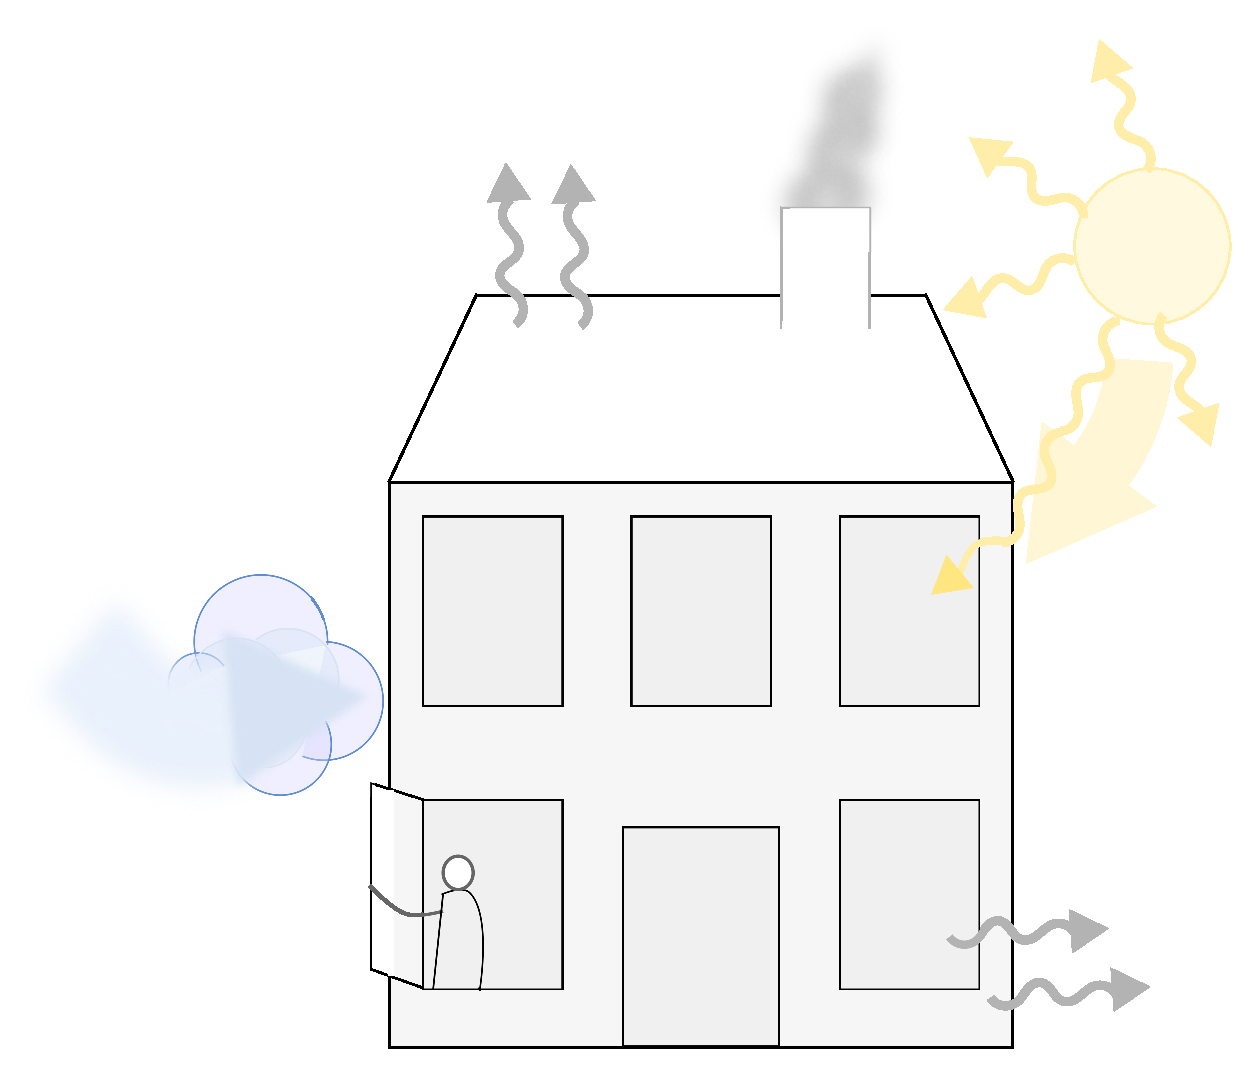
\includegraphics[scale=0.2]{../report/images/hus_framsida.eps}

    \vskip10pt

    Erik Ahlqvist, Ylva Dahl, Mats Lindström, Dan Ståby

    Institutionen för Teknisk Fysik

    29 maj, 2012

  \end{center}

}

\subsection{Syfte och bakgrund}

\begin{frame}{Bakgrund}

\frame{
  \begin{center}
    \includegraphics[scale=0.7]{../report/images/house.eps}
  \end{center}
}


\subsection{Byggnadsskal - väggar och tak}

%Definition av h-värde och U-värde

\frame{
       \frametitle{Några definitioner}
        \begin{align*}
        Q &= U\Delta T \\
        Q &= h(T-T_\infty)
        \end{align*}
        \begin{center}
          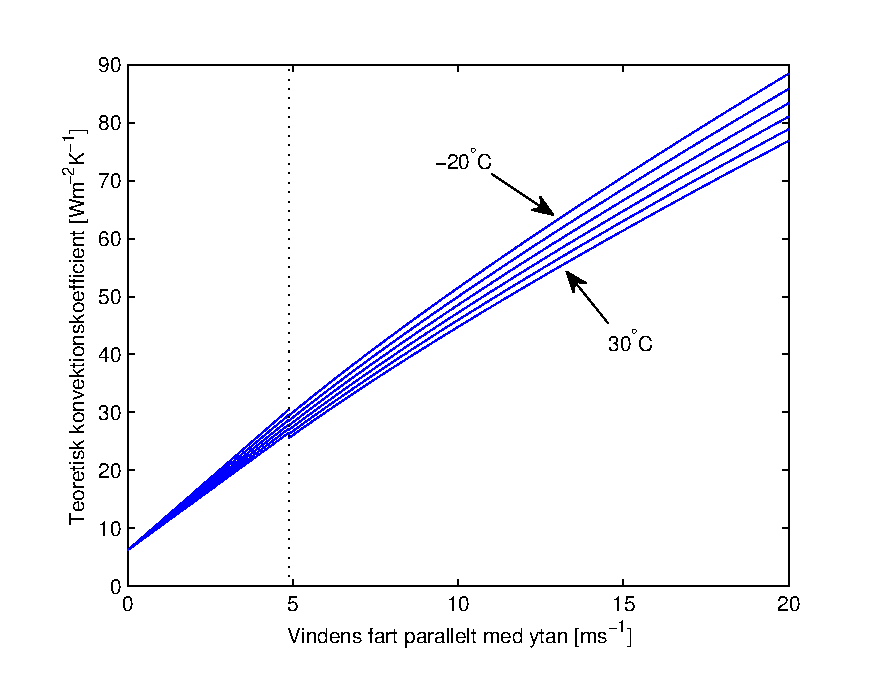
\includegraphics[scale=0.5]{../report/images/hvalues.eps}
        \end{center}
}


%Data för huset

\frame{
       \frametitle{Parametrar för huset}
        \begin{table}[hbtp]
        \centering
        \caption{Areor och U-värden för fastighetens klimatsköld. \emph{\color{red} Byta ut denna mot en mer talande figur?}}
        \label{tbl:uvalue}

        \begin{tabular}{|l|r|r|}
        \hline
        \textbf{Del} & \textbf{Area~$[\unit{m^2}]$} &\textbf{U-värde~$[\unit{W~m^{-2}~K^{-1}}]$} \\
        \hline
        Söderväggen &  151 & 1,186 \\ 
        Västerväggen & 61 & 1,186 \\
        Norrväggen & 290 & 0,279 \\
        Burspråket & 47 & 0,393 \\
        Taket & 257 & 0,171 \\
        \hline
        Fönster, söder & 109 & 1,0 \\
        Fönster, norr & 89 & 1,0 \\
        Fönster, tak & 8 & 1,0 \\
        \hline
        \textbf{Totalt} & \textbf{1012} & \textbf{0,6}\\
        \hline
        \end{tabular}
        \end{table}

}

\begin{frame}{Resultat}
 
\begin{figure}
        \begin{subfigure}[b]{0.48\textwidth}
                \centering
                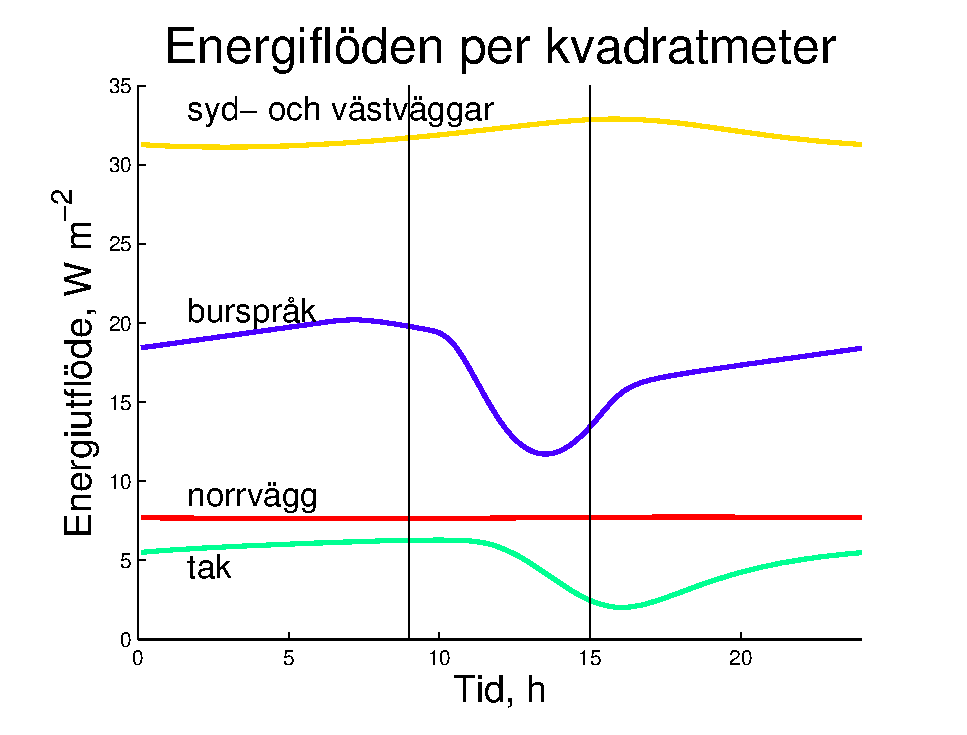
\includegraphics[width=\textwidth]{images/walls1.eps}
        \end{subfigure}
        \begin{subfigure}[b]{0.48\textwidth}
                \centering
                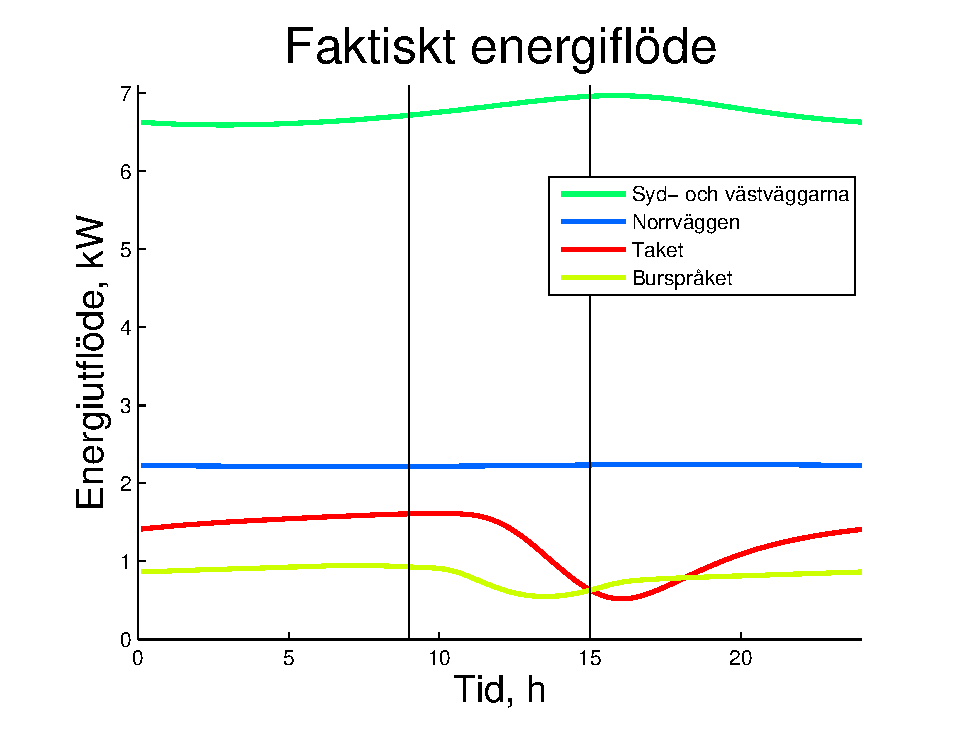
\includegraphics[width=\textwidth]{images/walls2.eps}
        \end{subfigure}
\end{figure}


\end{frame}



\subsection{Grunden}

\begin{frame}{Problemformulering, grunden}
\emph{\color{red} Inkludera bild över geometri och/eller triangulering?}
\begin{equation*}
k\mathbf{n}\cdot\nabla T(\mathbf{r},t) = 
\begin{cases}
0&\mbox{, för rand mot berg} \\
h[T_\infty(t)-T(t)]&\mbox{, för rand mot luft} \\
U[T_{inne} - T(t)]&\mbox{, för rand mot grund}
\end{cases}
\end{equation*}
\end{frame}

\begin{frame}{Energiflöden, grunden\\Hela året}

\begin{figure}[hpbt]
\centering
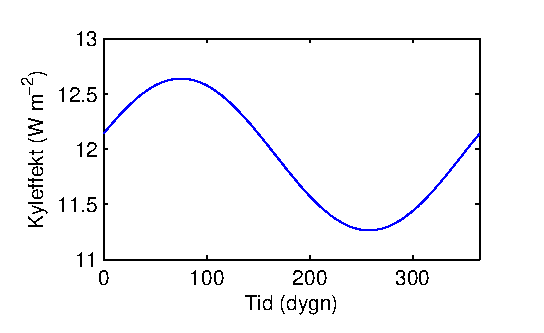
\includegraphics[height=5cm]{images/foundation.eps}
\caption*{Energiflödet genom grunden}
\end{figure}

\end{frame}


\subsection{Fönster}

\subsubsection{Solens position och intensitet}
\frame{
  % Bild på sol en solig decemberdag
}

\subsubsection{g-värden}
\frame{
  % Vinkelberoende
  % Hänvisa till artikeln
  % Åter till bild på solen, lägg till effektflödet
}

\subsubsection{Långvågsstrålning och approximationer}
\frame{
  % Förklaring av hur vi räknat med S-B:s lag
  % Diffus strålning och omedelbar reflektion borträknat
}

\subsubsection{Totalt genom fönster}
\frame{
  % Bild på totalen genom fönster - även värmeledning
}


\subsection{Slutsats och diskussion}

\begin{frame}{Sammanfattning av energiflöden\\En klar decemberdag}


\begin{figure}
        \begin{subfigure}[b]{0.55\textwidth}
                \centering
                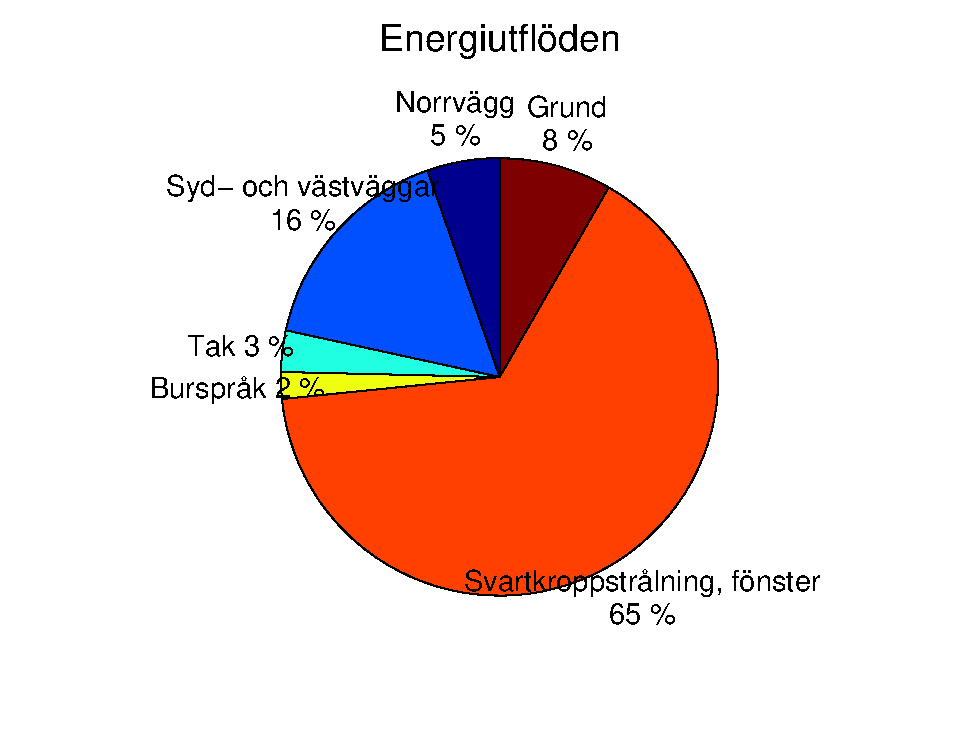
\includegraphics[width=\textwidth]{images/totalflow_out.eps}
                \caption*{Totalt 42 kWh/dygn \\ ~}
        \end{subfigure}
        \hskip-1.5cm
        	\uncover<2>{
        \begin{subfigure}[b]{0.55\textwidth}
                \centering
                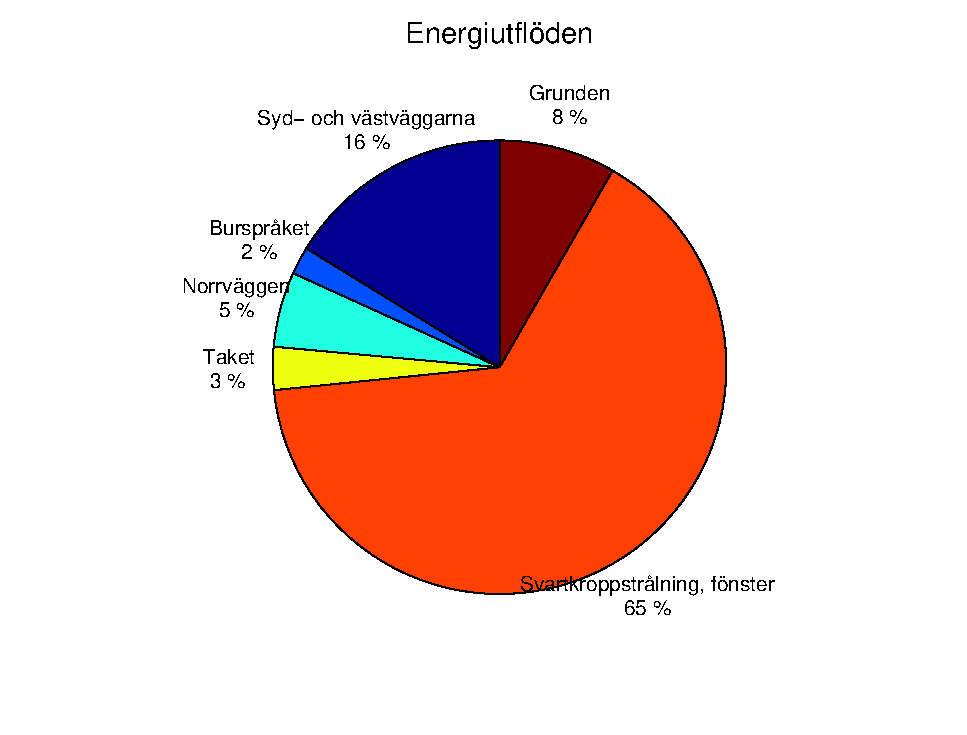
\includegraphics[width=\textwidth]{images/totalflow_in.eps}
                \caption*{Totalt 16 kWh/dygn \\+ tillförd energi}
        \end{subfigure}
        }
\end{figure}

\end{frame}


\subsection{Avslutande sammanfattning}

\frame{
\begin{center}
  \Huge{Väderstation?}
\end{center}
        \vskip1.3cm
\uncover<2>{
\begin{center}
  \color{red}{\Huge{Nej!}}
\end{center}

}
}

\end{document}
